% Befehl \fibelvorstellung: Erstellt die Vorstellung eines FSlers mit Bild
%	Parameter #1: Bild (wrapfigure)
%	Parameter #2: Text
\newcommand{\fibelvorstellung}[2]{%
	\begin{minipage}{\columnwidth}
		% Kein Abstand vor bzw. nach Bildern bei wrapfigure
		\setlength{\intextsep}{0cm}
		% geringfügiger Abstand zwischen Paragraphen
		\setlength{\parskip}{0.5ex}
		#1
		#2
		\vspace{0.5ex}
	\end{minipage}
	
	\vspace{5ex plus 2ex minus 1ex}
}
\newlength{\fibelstdlen}
\setlength{\fibelstdlen}{3.7cm}

\section{Der Fachschaftsrat~(FSR) Physik stellt sich vor}
\begin{multicols}{2}
\small


\fibelvorstellung{
	\begin{wrapfigure}{l}{0cm}
		\includegraphics[width=\fibelstdlen]{res/vorstellungsfotos/michael_te_vrugt}
	\end{wrapfigure}
}
{
Hi, ich bin Michael und stehe kurz vor dem Ende meiner Promotionen in Physik und Philosophie. In der Fachschaft bin ich seit Jahren aktiv. 
Bei Fragen zu Philosophie, einem Auslandsjahr, Doppelstudium oder Stipendium - und natürlich auch allem anderen - seid ihr bei mir genau richtig. Ansonsten wünsche ich euch viel Spaß der O-Woche, und vielleicht sieht man sich mal bei einer Fachschaftssitzung. :)
}

\vspace{-0.4cm}

\fibelvorstellung{
	\begin{wrapfigure}{r}{0cm}
		\includegraphics[width=\fibelstdlen]{res/vorstellungsfotos/Hauke_neu.jpg}
	\end{wrapfigure}
}
{
Moin, ich heiße Hauke und bin seit 2016 an der Uni und momentan Vorsitzender der Fachschaft. Als Erasmus Student war ich in Sevilla (Spanien) und in Münster bin ich u.\,A. für die Evaluation der Lehre zuständig. 
Euch ein herzliches Willkommen in Münster!
}

\vspace{-0.1cm}

\fibelvorstellung{
	\begin{wrapfigure}{l}{0cm}
		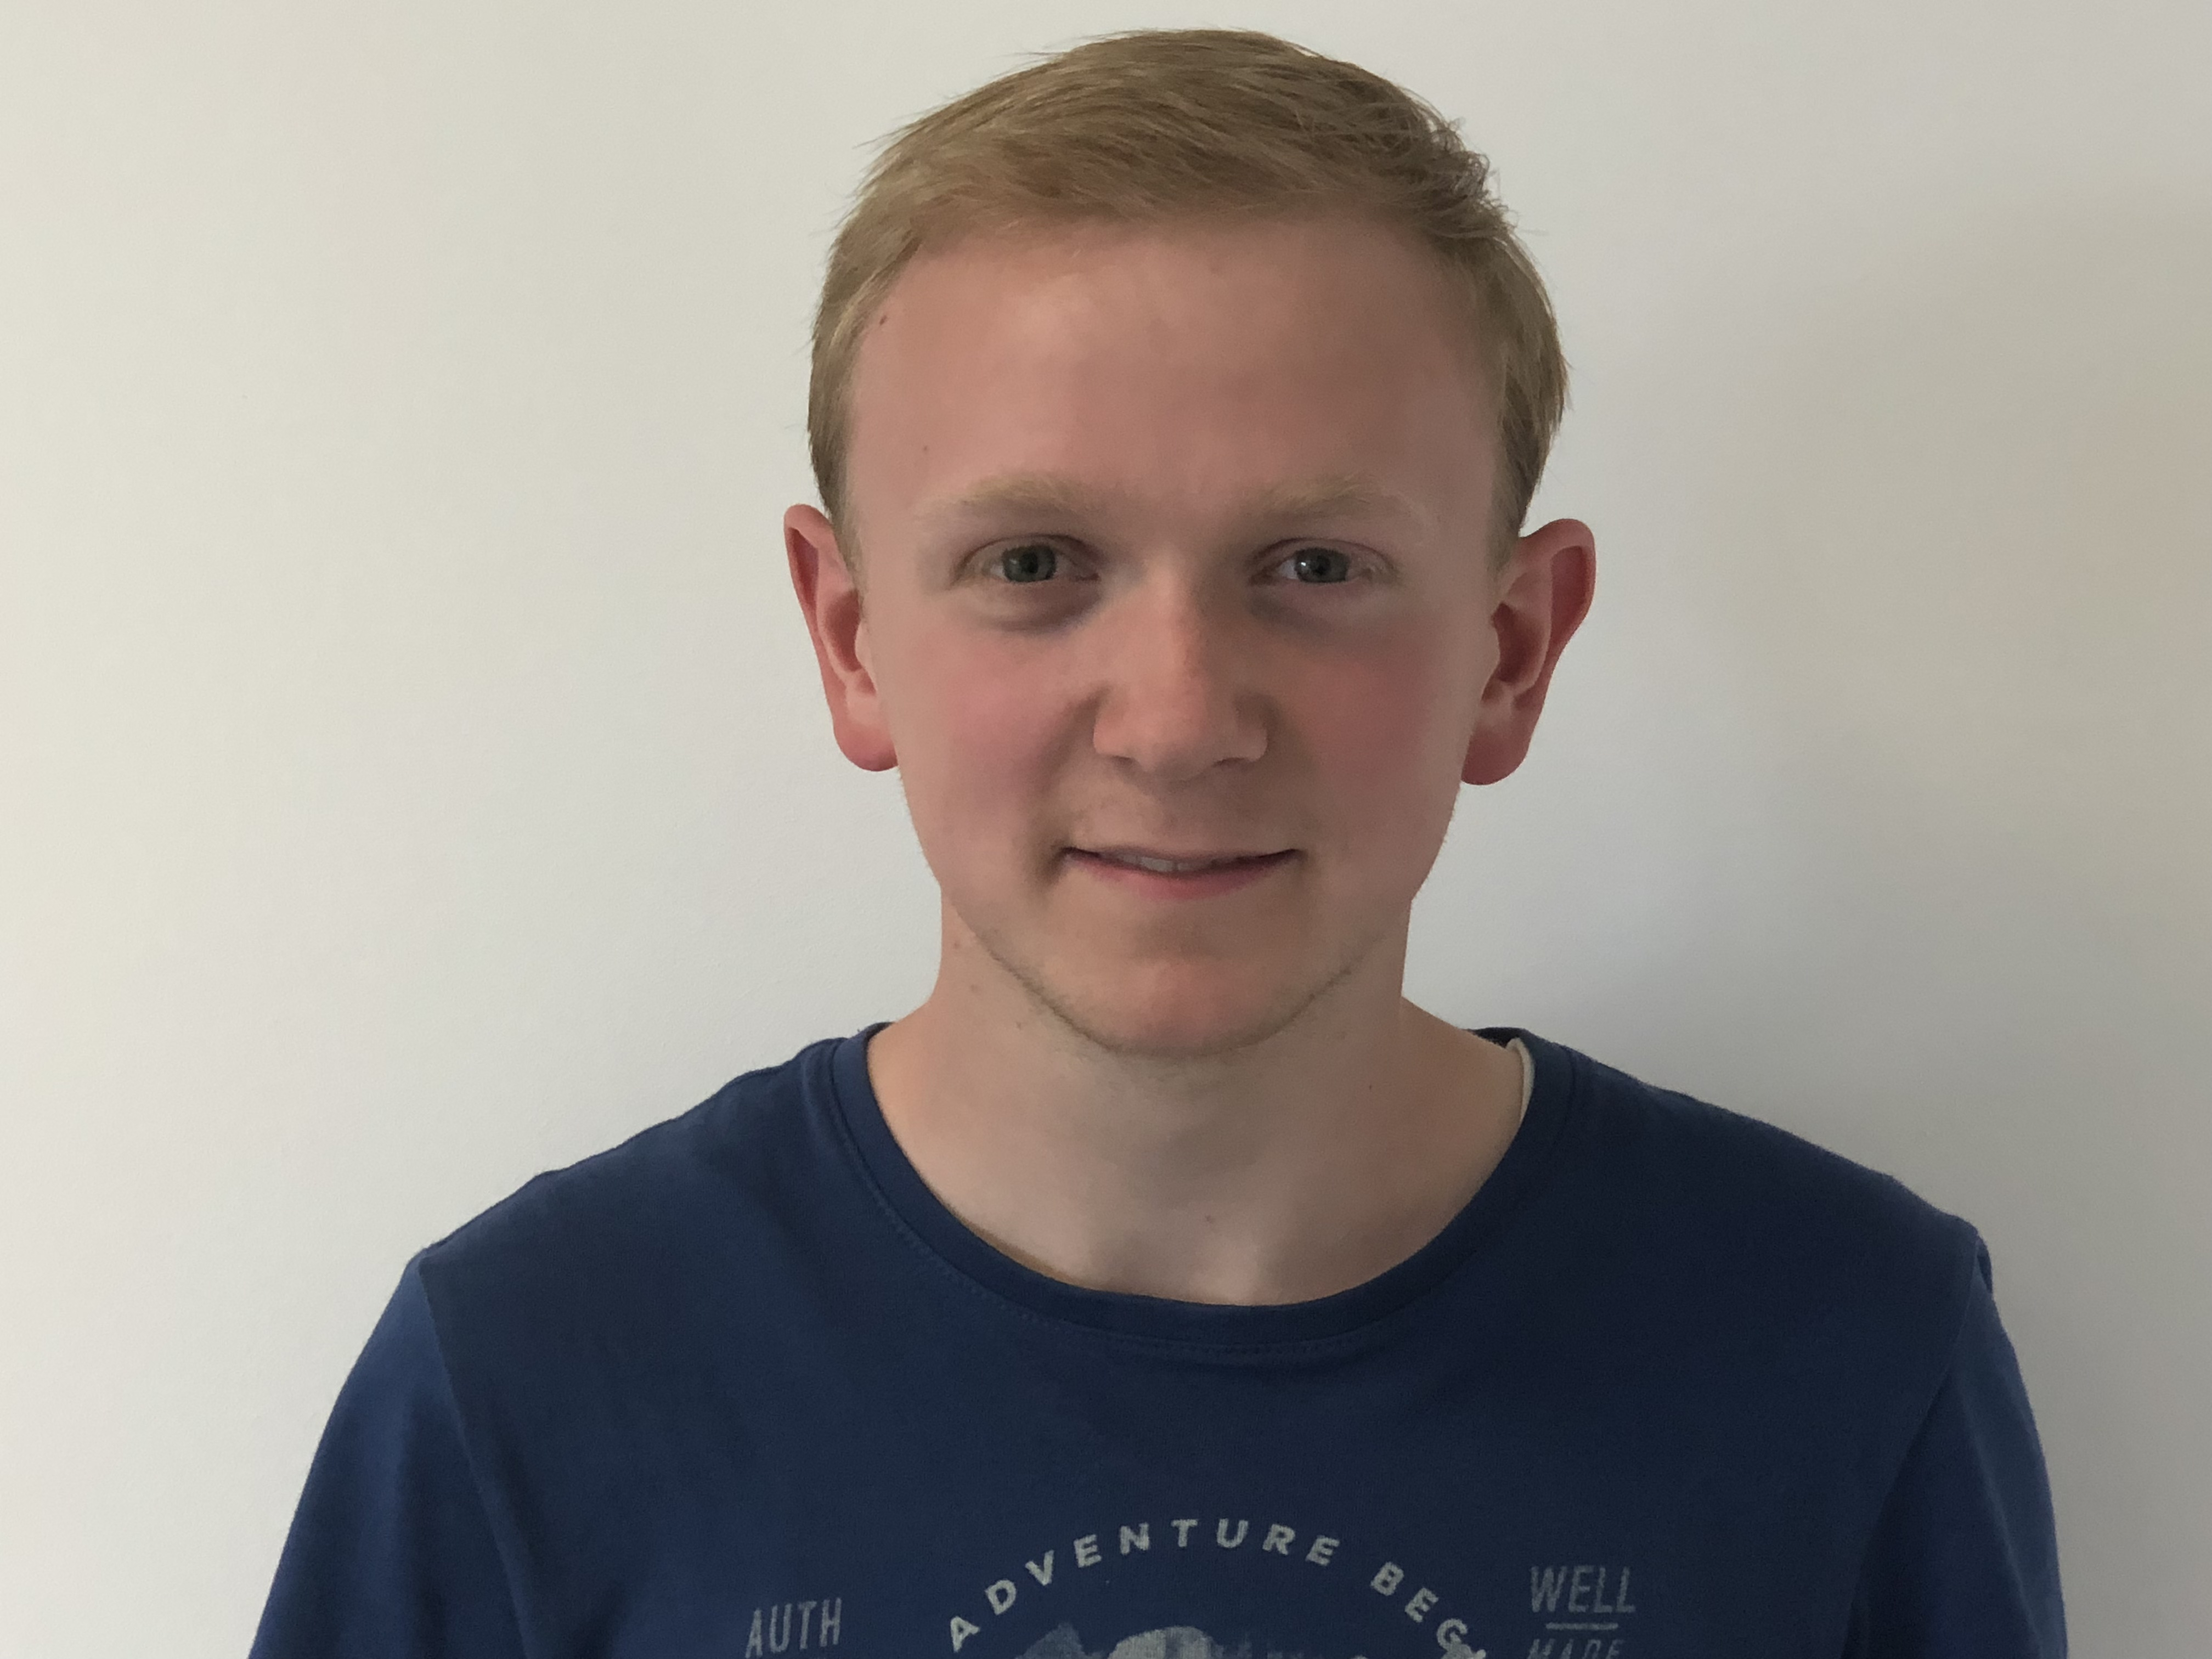
\includegraphics[width=\fibelstdlen]{res/vorstellungsfotos/Fotos Selbstvorstellungstexte Fibel/tim_stellhorn.jpg}
	\end{wrapfigure}
}
{
Hej, ich bin Tim und studiere Physik im Master. In der Fachschaft bin ich Finanzer, aber auch besonders zu Auslandsaufenthalten kann ich eure Fragen beantworten, denn ich war selber für ein Jahr in Lund in Schweden. 
Für die O-Woche wünsche ich euch viel Spaß und hoffe, dass ihr viele andere Erstis kennen lernt, denn mit Leidensgenossen lassen sich die ganzen Übungszettel deutlich besser rechnen. Doch lasst euch davon nicht abschrecken! Erstmal habt eine schöne Zeit und vielleicht läuft man sich ja mal in der Uni über den Weg, zum Beispiel beim Spieleabend der Fachschaft. ;-)
}

\fibelvorstellung{
	\begin{wrapfigure}{l}{0cm}
		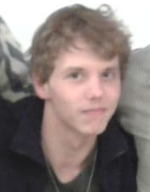
\includegraphics[width=\fibelstdlen]{res/vorstellungsfotos/Marius_cut.PNG}
	\end{wrapfigure}
}
{
Hi, ich bin Marius und heiße euch ebenfalls herzlich willkommen hier in Münster. Wenn ihr die Stadt noch nicht richtig kennt, dann freut euch darauf, sie kennenzulernen. 
Das Studium wird zwar zwischendurch hart, aber lasst euch trotzdem nicht die Freude dran nehmen. ¡Mucha suerte!\footnote{\url{https://www.youtube.com/watch?v=iik25wqIuFo}}
}


\vspace{-0.4cm}

\fibelvorstellung{
	\begin{wrapfigure}{l}{0cm}
		\includegraphics[width=\fibelstdlen]{res/vorstellungsfotos/benedikt_bieringer.png}
	\end{wrapfigure}
}
{
Hallo zusammen! Mein Name ist Benedikt. In der Fachschaft beschäftige ich mich unter anderem mit Computergrafik/Design. 
Programmieren und Schwimmen sind nur zwei meiner weiteren Freizeitbeschäftigungen. 
In meinen mittlerweile schon 16~Semestern Fachschafts- und Studienerfahrung kann ich euch aber auch bei einer ganzen Reihe weiterer Fragen weiterhelfen.
}

\vspace{-0.5cm}

\fibelvorstellung{
	\begin{wrapfigure}{r}{0cm}
		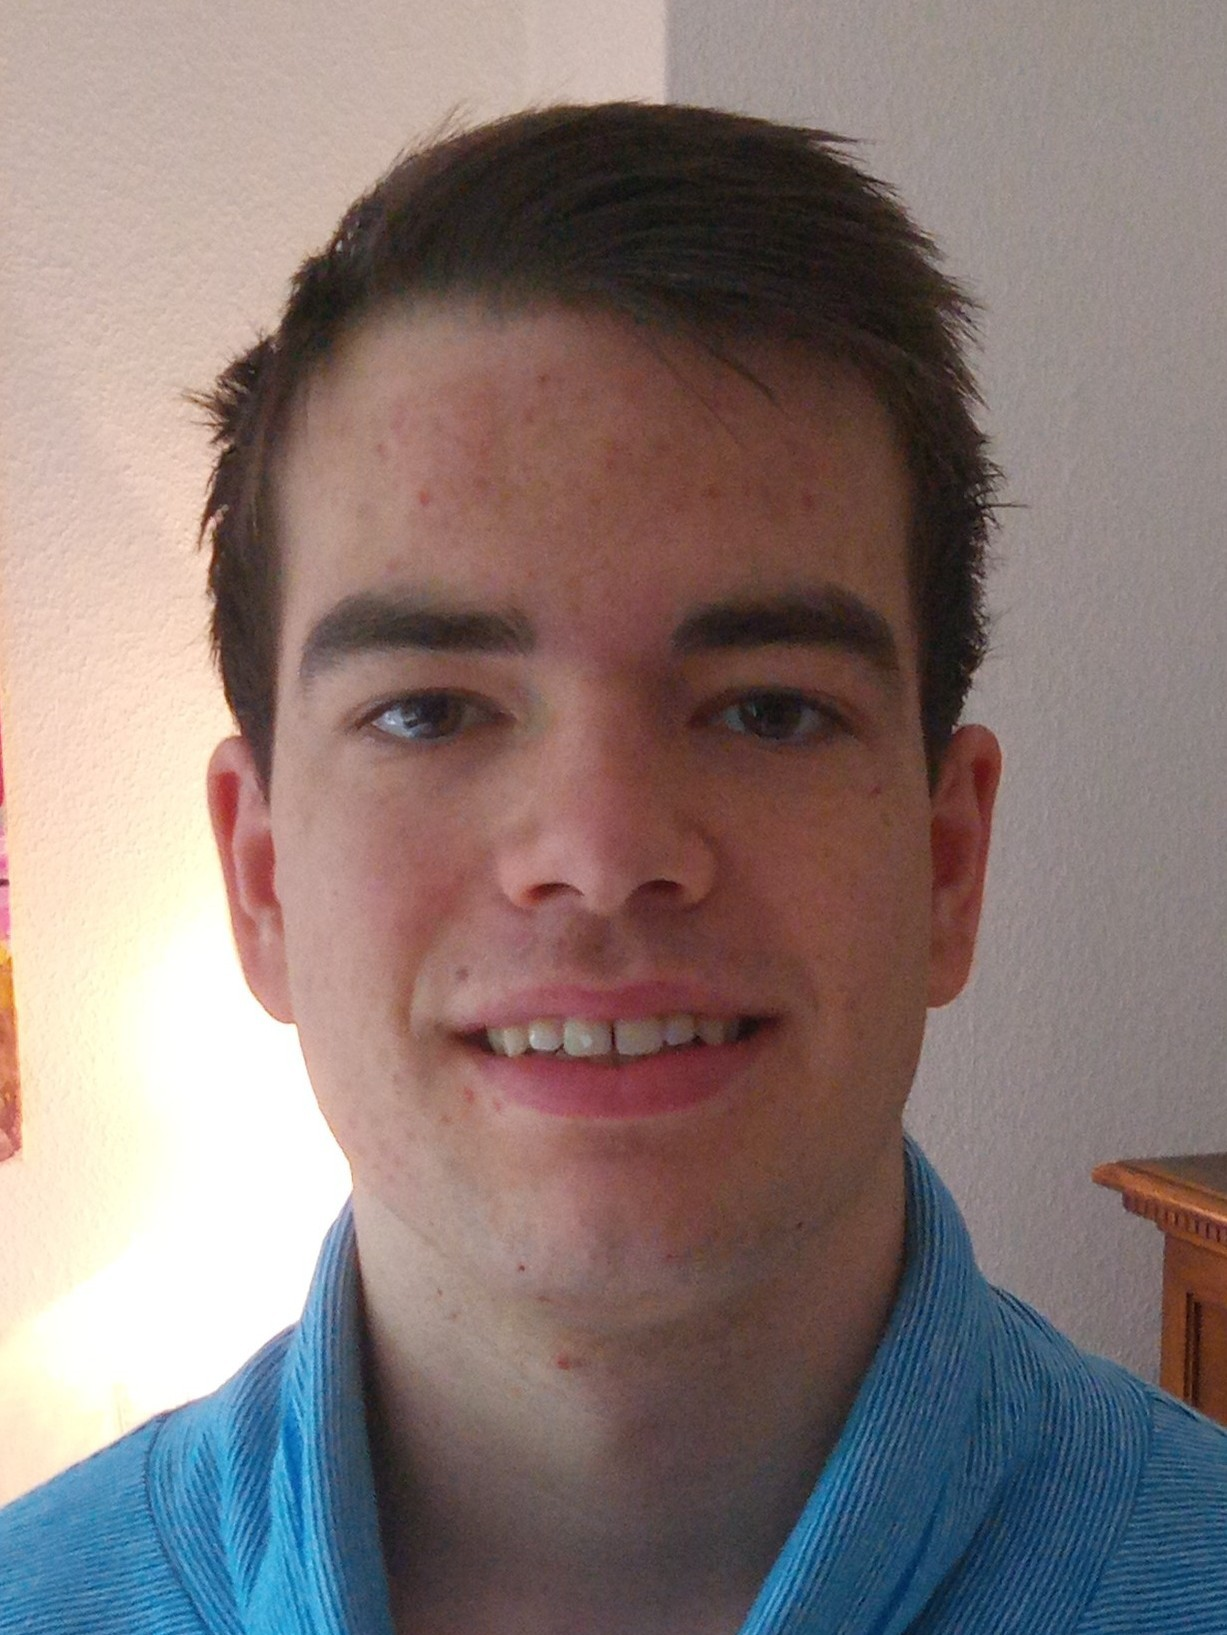
\includegraphics[width=\fibelstdlen]{res/vorstellungsfotos/Fotos Selbstvorstellungstexte Fibel/Lambert.jpg}
	\end{wrapfigure}
}
{
Hallo, ich bin Lambert und jetzt im 5. Semester meines Physikbachelors. Ich bin u.a. mitverantwortlich für die Evaluation der Lehre, helfe im O-Wochen-Team
und weiß zu viel über Star Wars und Bücher von Neil Gaiman. Mit Fragen zu allem möglichen könnt ihr euch gerne an mich wenden.
Willkommen in Münster und einen schönen Studiumsbeginn!
}

\vspace{-1.1cm}

\fibelvorstellung{
	\begin{wrapfigure}{l}{0cm}
		\includegraphics[width=\fibelstdlen]{res/vorstellungsfotos/Jasemin.jpg}
	\end{wrapfigure}
}
{
Hey\textasciicircum\textasciicircum \\
Ich bin Jasemin und studiere Physik und Sozialwissenschaften auf Lehramt. In der Fachschaft bin ich für die O-Woche und die Ersti-Fahrt verantwortlich.
Wenn ihr Fragen zum Lehramt habt, könnt ihr gerne auf mich zukommen.
Ich wünsche euch viel Spaß in eurem Studium.
}

\fibelvorstellung{
	\begin{wrapfigure}{l}{0cm}
		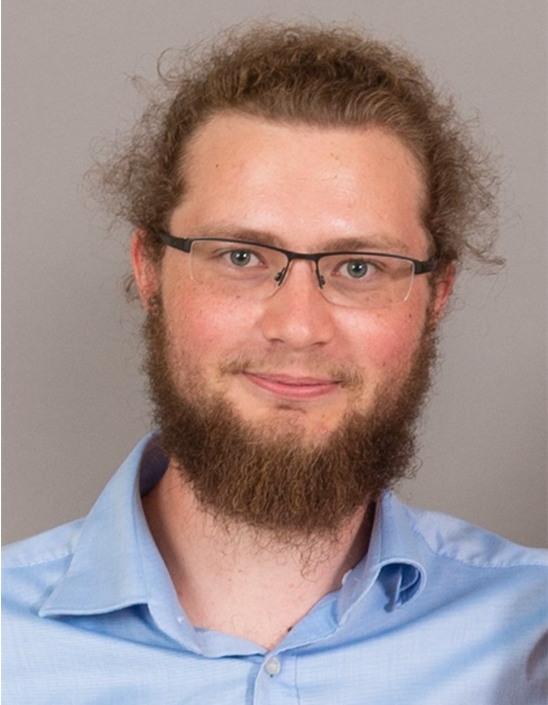
\includegraphics[width=\fibelstdlen]{res/vorstellungsfotos/Ali_cut.PNG}
	\end{wrapfigure}
}
{
Hallo Welt! Ich verkehre unter den Namen Alexander, Alekschander, Alex, Xander, Ali, Puck und Pucky. Bald geht es bei mir mit der Promotion los. 
In der Fachschaft beschäftige ich mich mit IT-Administration. Entsprechend kann ich bei Fragen zu Physik und Technik gerne helfen. \texttt{\kern-0.25ex\raisebox{0.25ex}{\rotatebox{45}{\raisebox{-.75ex}\grqq\kern-1.5ex\rotatebox{-90})}}\kern-0.5ex}
}

% \vspace{-0.3cm}

\fibelvorstellung{
	\begin{wrapfigure}{r}{0cm}
		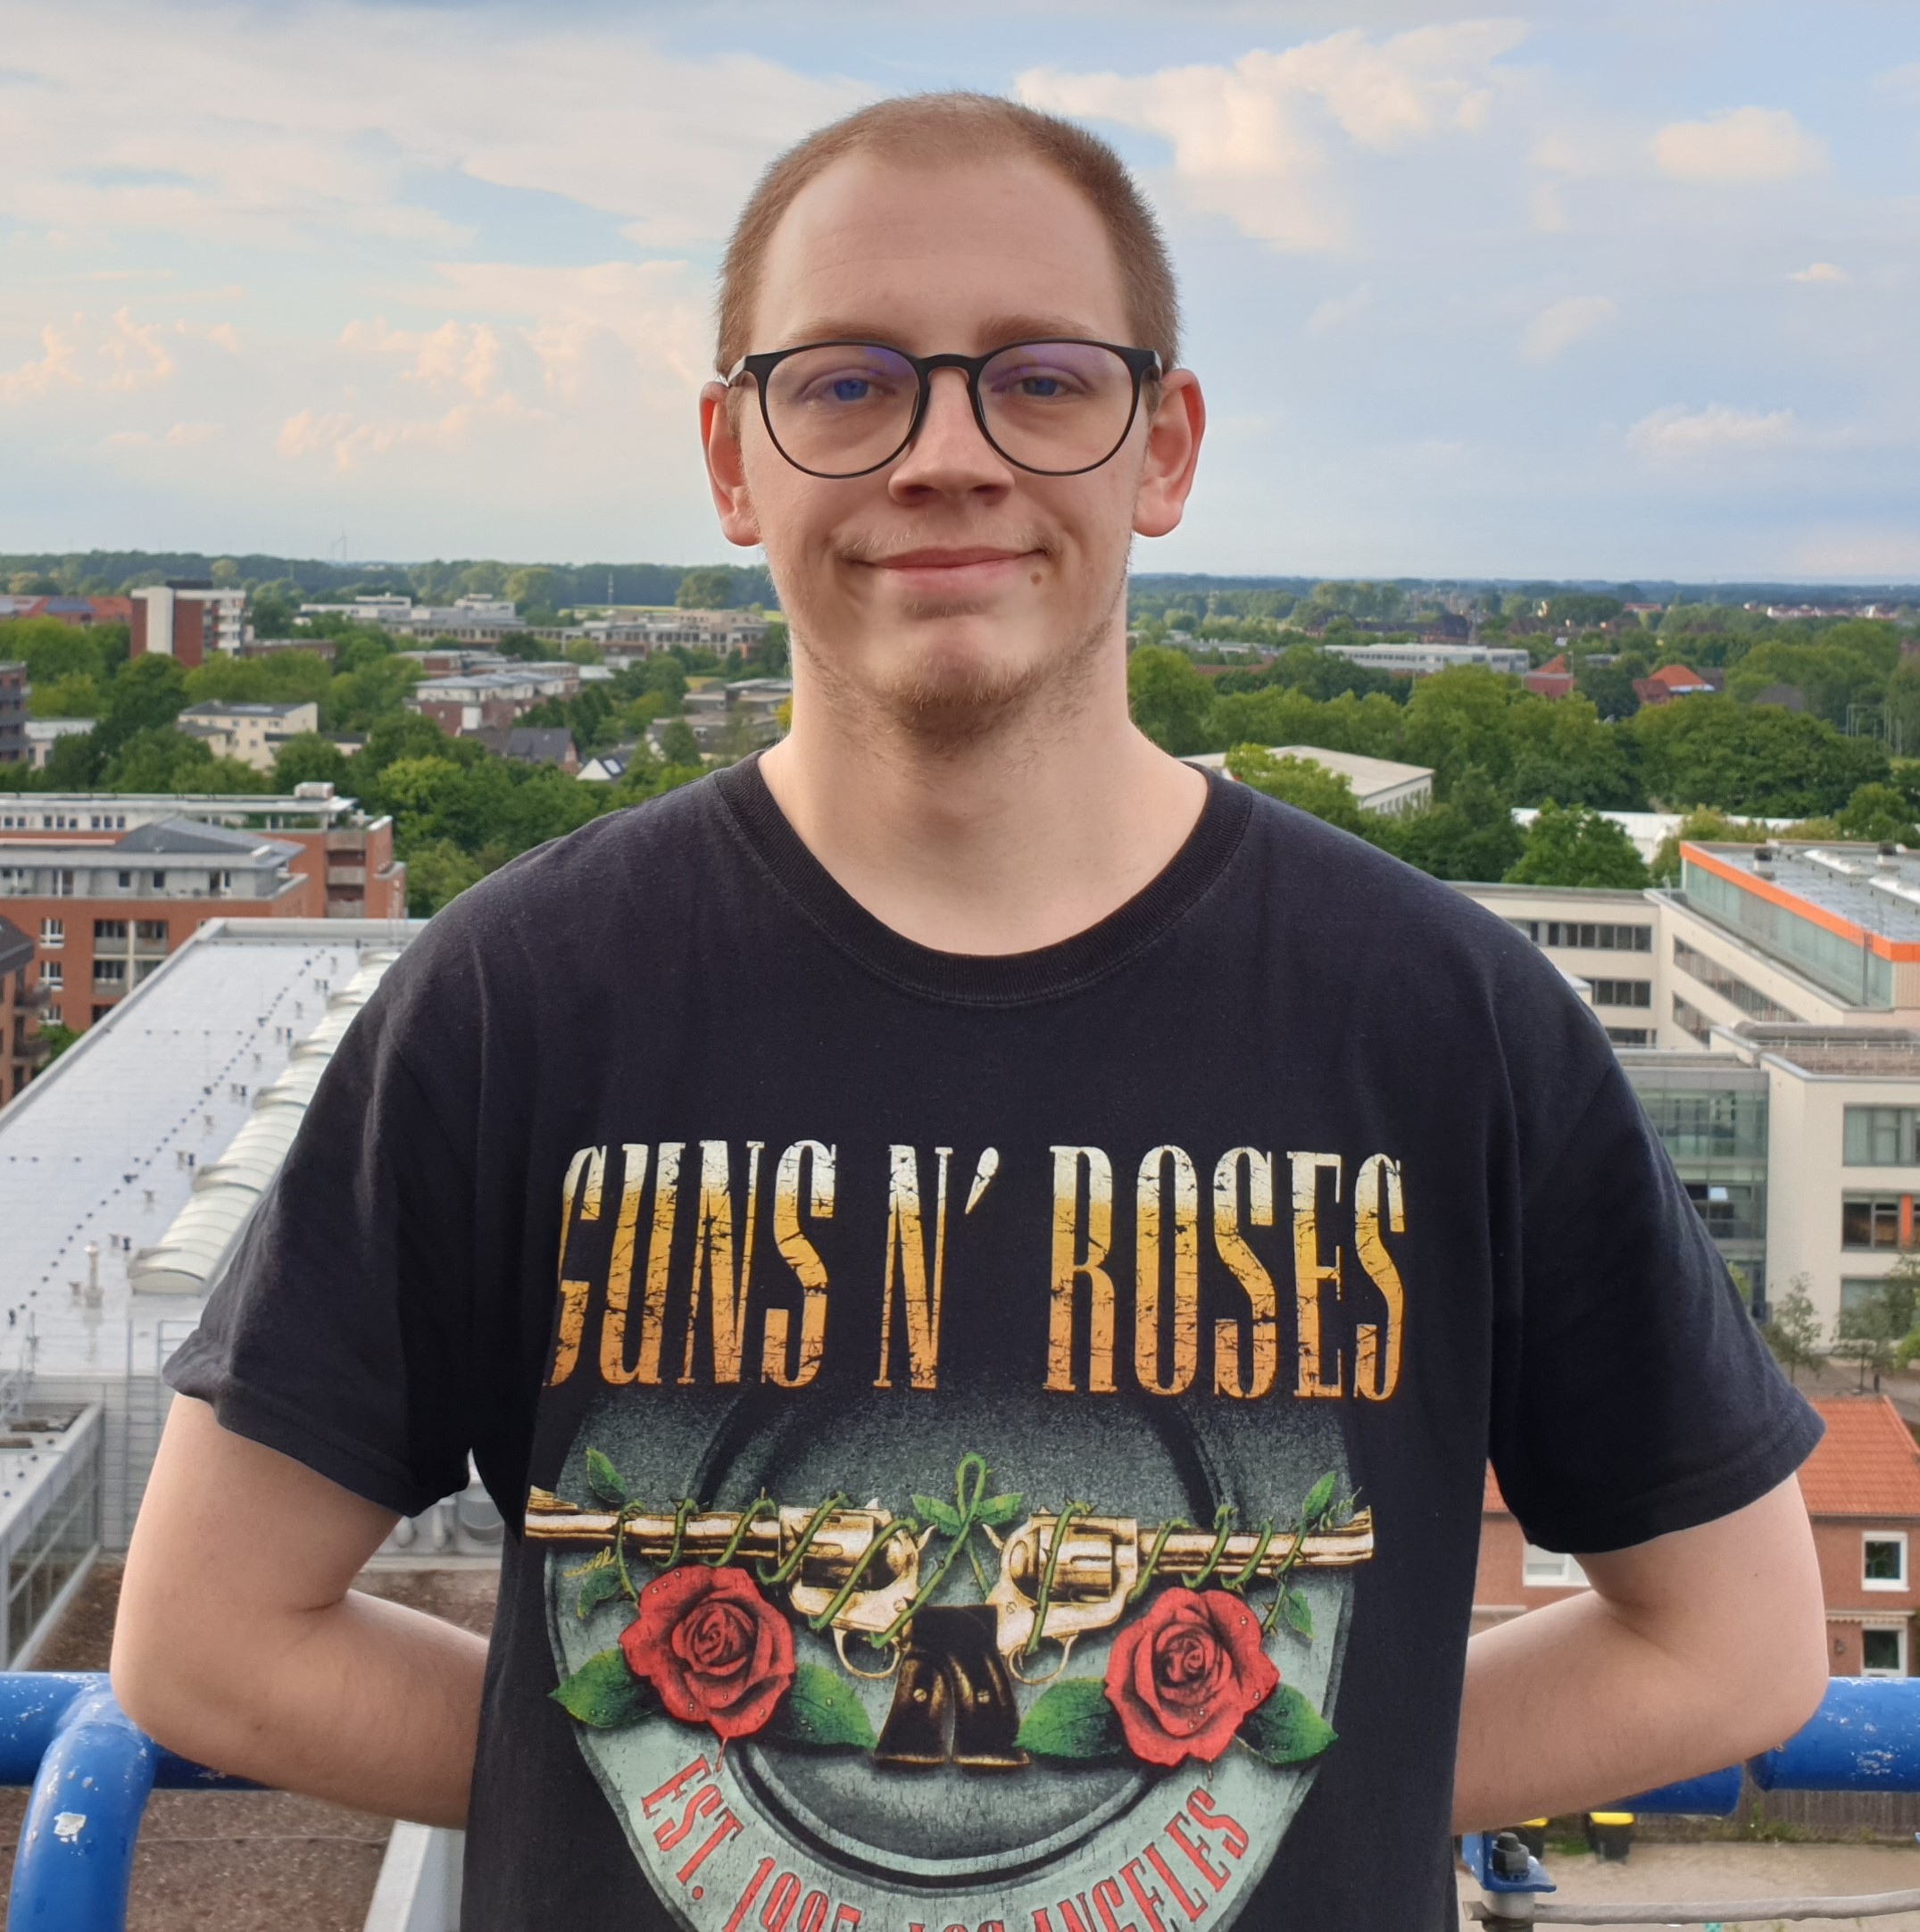
\includegraphics[width=\fibelstdlen]{res/vorstellungsfotos/Alexander_T_cut.jpg}
	\end{wrapfigure}
}
{
Hi, ich bin Alexander und seit dem Sommersemester 2022 Mitglied in der Fachschaft. Ich organisiere unter anderem die Ersti-Fahrt, schreibe an dieser Fibel und bin für die IT zuständig. Ich heiße euch herzlich willkommen an der Uni Münster und wünsche einen guten Start in das Studium!
}

\vspace{-1.1cm}

\fibelvorstellung{
	\begin{wrapfigure}{r}{0cm}
		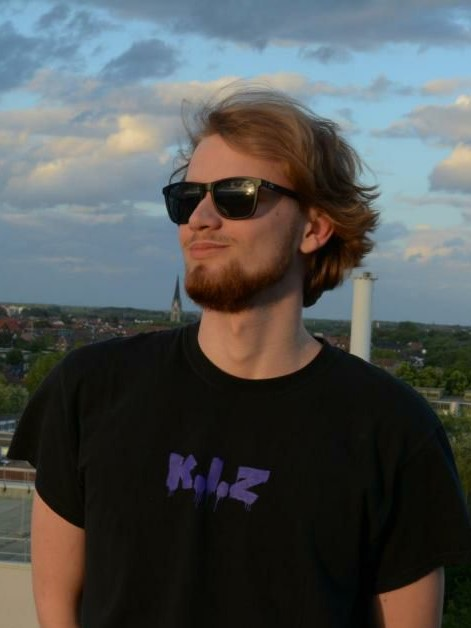
\includegraphics[width=\fibelstdlen]{res/vorstellungsfotos/Philipp_cut.JPG}
	\end{wrapfigure}
}
{
Moin Servus, \\ 
Ich bin der Phil und studiere mittlerweile seit drei Jahren Physik. Im Moment arbeite ich an meiner Bachelorarbeit sowie ein paar letzten Prüfungen. In der Fachschaft bin ich allerdings erst seit einem Jahr aktiv und kümmere mich hier unter Anderem um die Nikolaus-Aktion, im Dezember seht ihr mich dann hoffentlich als Nikolaus im Hörsaal. Bis dahin noch eine schöne O-Woche und ein guten Start in den Studienalltag. 
}

\vspace{0.3cm}

\fibelvorstellung{
	\begin{wrapfigure}{l}{0cm}
		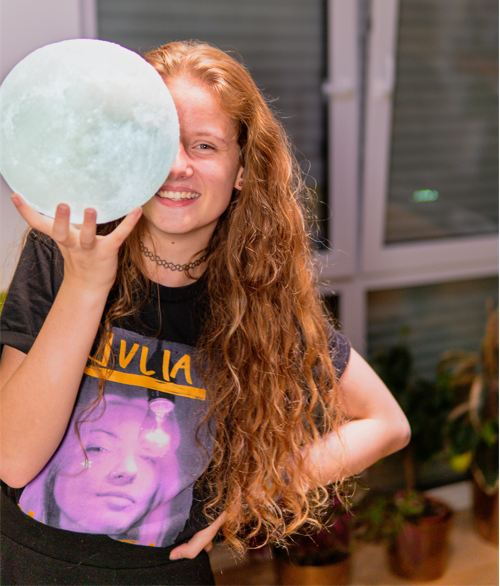
\includegraphics[width=\fibelstdlen]{res/vorstellungsfotos/Eva_cut.PNG}
	\end{wrapfigure}
}
{
Hey, ich heiße Eva und schreibe momentan an meiner Bachelorarbeit. Seit dem Sommersemester 2020 bin ich in der Fachschaft und nun stellvertretende Vorsitzende. Außerdem betätigte ich mich im Design-Team und in der Öffentlichkeitsarbeit. 
Ich wünsche Euch einen tollen Start ins Studium! PS: Über ein freundliches "Hallo" (auf dem Gang, im Vorbeigehen) freue ich mich immer.
} 

\vspace{0.1cm}

\fibelvorstellung{
	\begin{wrapfigure}{r}{0cm}
		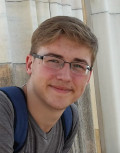
\includegraphics[width=\fibelstdlen]{res/vorstellungsfotos/christoph_wesseler.jpeg}
	\end{wrapfigure}
}
{
Sehr geehrte Erstis: Moin!
Ich bin Christoph und studiere im Master Physik. In der Fachschaft bin ich im O-Wochen Team und beim Sommerfest tätig. Wenn Ihr Fragen habt, z.B zur O-Woche oder zum etwas Chaotischen Alltag an der Uni, immer her damit, es lebe das Chaos! :D 
Ich wünsche euch allen eine schöne O-Woche und hoffe man sieht sich mal in der Fachschaft.
}



\fibelvorstellung{
	\begin{wrapfigure}{r}{0cm}
		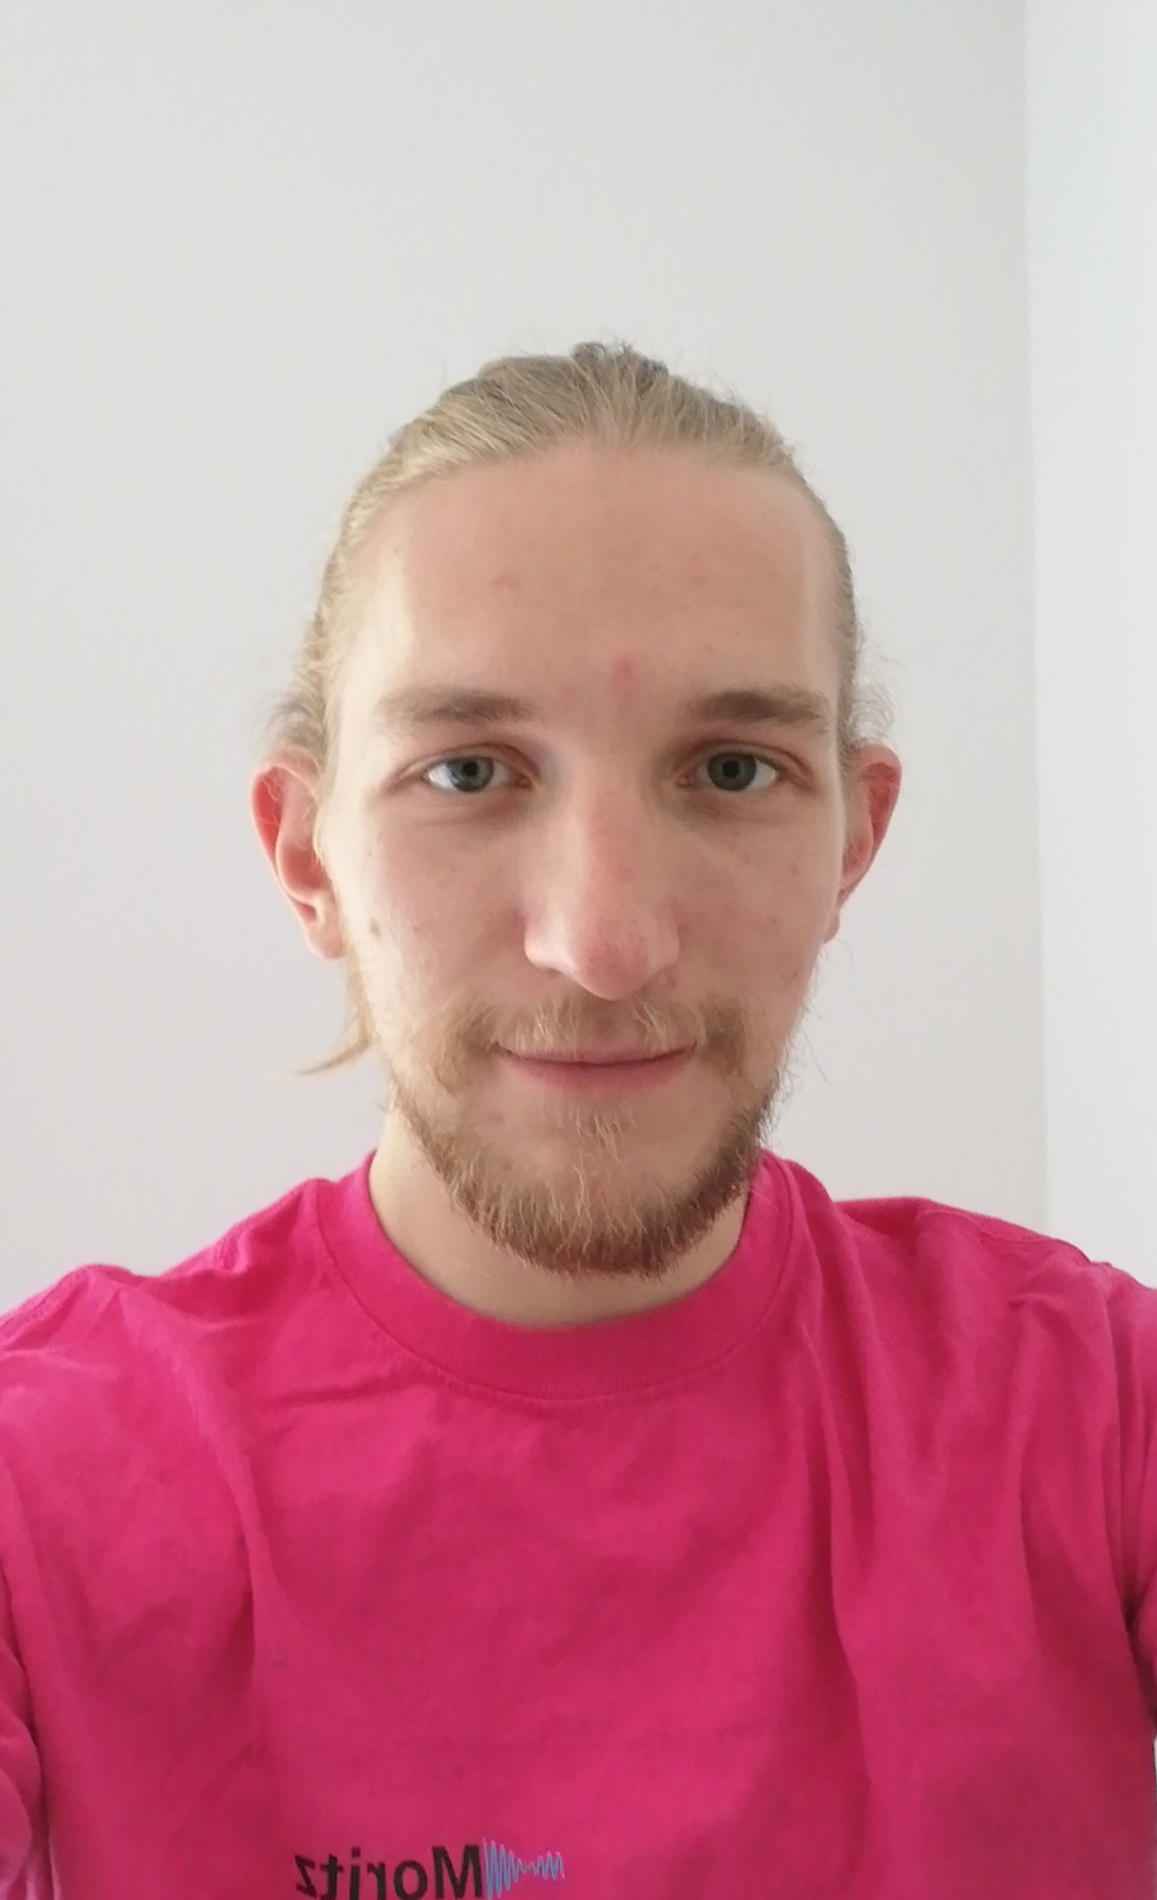
\includegraphics[width=\fibelstdlen]{res/vorstellungsfotos/Moritz.jpg}
	\end{wrapfigure}
}
{
Moin, ich bin Moritz und jetzt seit 5 Semestern in der Fachschaft. Ich studiere im Zwei-Fach-Bachelor Physik und Chemie, bei Fragen zum Lehramtsstudium dürft ihr mich also gerne ansprechen. 
Ich wünsche euch einen erfolgreichen Start ins Studium und insbesondere für die ZFB möglichst wenig Überschneidungen in euren Stundenplänen. :)
}

\fibelvorstellung{
	\begin{wrapfigure}{l}{0cm}
		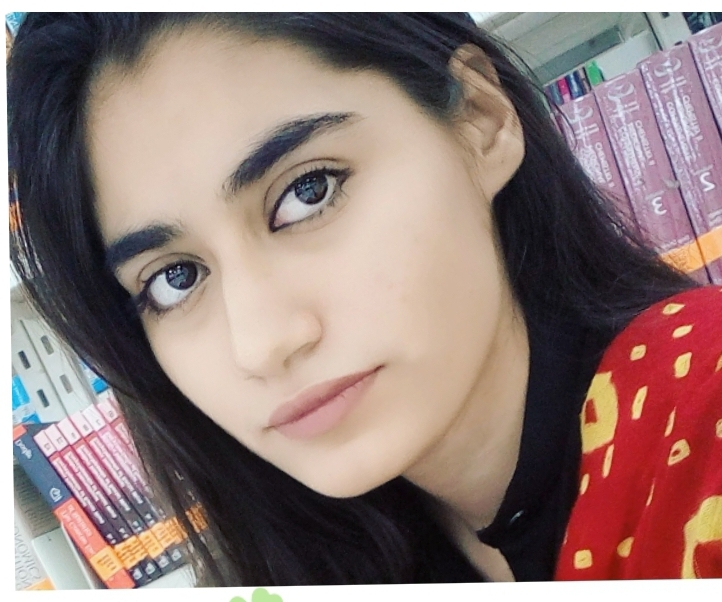
\includegraphics[width=\fibelstdlen]{res/vorstellungsfotos/Saba.jpg}
	\end{wrapfigure}
}
{
Hi, ich bin Saba Ahmed Cheema und studiere Physik auf Master. Zur Zeit bin ich auch Mitglied einer Berufungskommission einer Professur zur Photonik. Ich wünsche euch einen guten Start in's Studium. 
}



%
% \begin{center}
% 	\includegraphics[width=\columnwidth]{res/fsphys_logo.pdf}
% \end{center}
%
%
%

% \vspace{6ex}

% \fibelvorstellung{
% 	\begin{wrapfigure}{r}{0cm}
% 		\includegraphics[width=\fibelstdlen]{res/vorstellungsfotos/fritz.png}
% 	\end{wrapfigure}
% }
% {
% Hallo, ich bin Fritz und bin schon  in der Fachschaft Physik.
% Die Mannschaft hier ist echt genial aufgestellt. Dadurch macht es richtigen Spaß, ein aktiver Teil der Universität % Münster zu sein.
% Ich kann dir nur empfehlen: Mach' mit und verändere die Uni!
% }


\end{multicols}

% \vspace{20ex}
